\subsection{Fixed-Target Posterior Assessment}
\label{sec:supp-mti-posterior-assessment}
The computation study contains 360 simulation samples, with five in each
distribution and sample-size/content setting, and ten application training
partitions, one for each response and partition scheme. An additional 86
samples retain the extreme-content and extreme-tilt cases examined with
the augmented sampler. All calculations use the archived ECM-selected
\(q,\delta\), \(\omega_{\mathrm R}=1\), and \(\lambda=10^{-4}\).
Four marginal slice-within-Gibbs chains use 2000 burn-in and 4000 retained
iterations per sample. Every one of the 456 samples has \(\widehat R<1.01\),
bulk and tail effective sample sizes above 400, and mean Monte Carlo error
below 5\% of posterior standard deviation. The largest \(\widehat R\)
is 1.0031; the smallest bulk and tail effective sample sizes are 1781 and 2824.
These diagnostics use ordered endpoints, width, and midpoint
\citep{VehtariEtAl2021Rhat}. Quantile-specific Monte Carlo errors are
recorded separately. All primary means, medians, and credible endpoints
meet the additional 1\%-of-median-width reporting resolution in 125 samples;
the remaining samples retain their numerical-error summaries for review.

The original augmented sampler was run on 174 of these samples, of which
20 met its original diagnostic criteria at the same chain length. One
4000-iteration extension per chain was applied to 18 borderline samples.
The marginal updates preserve the same generalized posterior while reducing
the dependence associated with latent-scale augmentation in these examples.
Posterior summaries from poorly mixed augmented chains are retained as
diagnostics. Comparisons of posterior means are restricted to original
chain sets meeting the stated diagnostic criteria. Both samplers use
identical observations and fixed targets.

Writing \(J_{\mathrm{ECM}}\) for the archived objective and
\(J_{\min}\) for the independently minimized value, the relative gap
\[
\frac{J_{\mathrm{ECM}}-J_{\min}}{\max\{1,|J_{\mathrm{ECM}}|\}}
\]
exceeds \(10^{-4}\) in 96 samples.
Of these, 94 have tilts outside the empirical limits. This comparison
assesses the optimization accuracy of the specified finite iteration;
the independent reference attains a relative objective bound below
\(5\times10^{-13}\) in every sample. Among the 20 original augmented
chain sets meeting their stated diagnostics, 77 of 80 posterior-mean
comparisons lie within twice the combined Monte Carlo standard error.
The largest standardized difference is 2.47.

Figure~\ref{fig:supp-mti-posterior-width} separates a finite ECM iterate,
a separately minimized penalized-loss reference, and posterior uncertainty
at the same fixed target. This sample-dependent minimum serves only to
assess optimization accuracy; the tolerance study retains its original
ECM estimates. At an empirical limiting tilt, one endpoint can move beyond the
data with little loss change, leaving the Gaussian prior to constrain
posterior dispersion. Slightly outside the limiting range, further movement
can reduce the unpenalized loss. These effects explain why improved mixing
can reveal substantial width uncertainty even when a short ECM sequence
appears stable. A change to the prior, learning rate, or target-selection
rule requires a separately specified tolerance calibration.

A local prior-sensitivity calculation reweights the saved draws to
Gaussian root variances equal to one half and one tenth of the original
variance. It records weight effective sample size and the Monte Carlo
error of each weighted mean. The results show substantial prior influence
in many limiting-tilt examples. Inadequate importance overlap leaves
some sensitivity estimates unresolved; these estimates are excluded
from substantive comparisons.

\begin{figure}[!htbp]
\centering
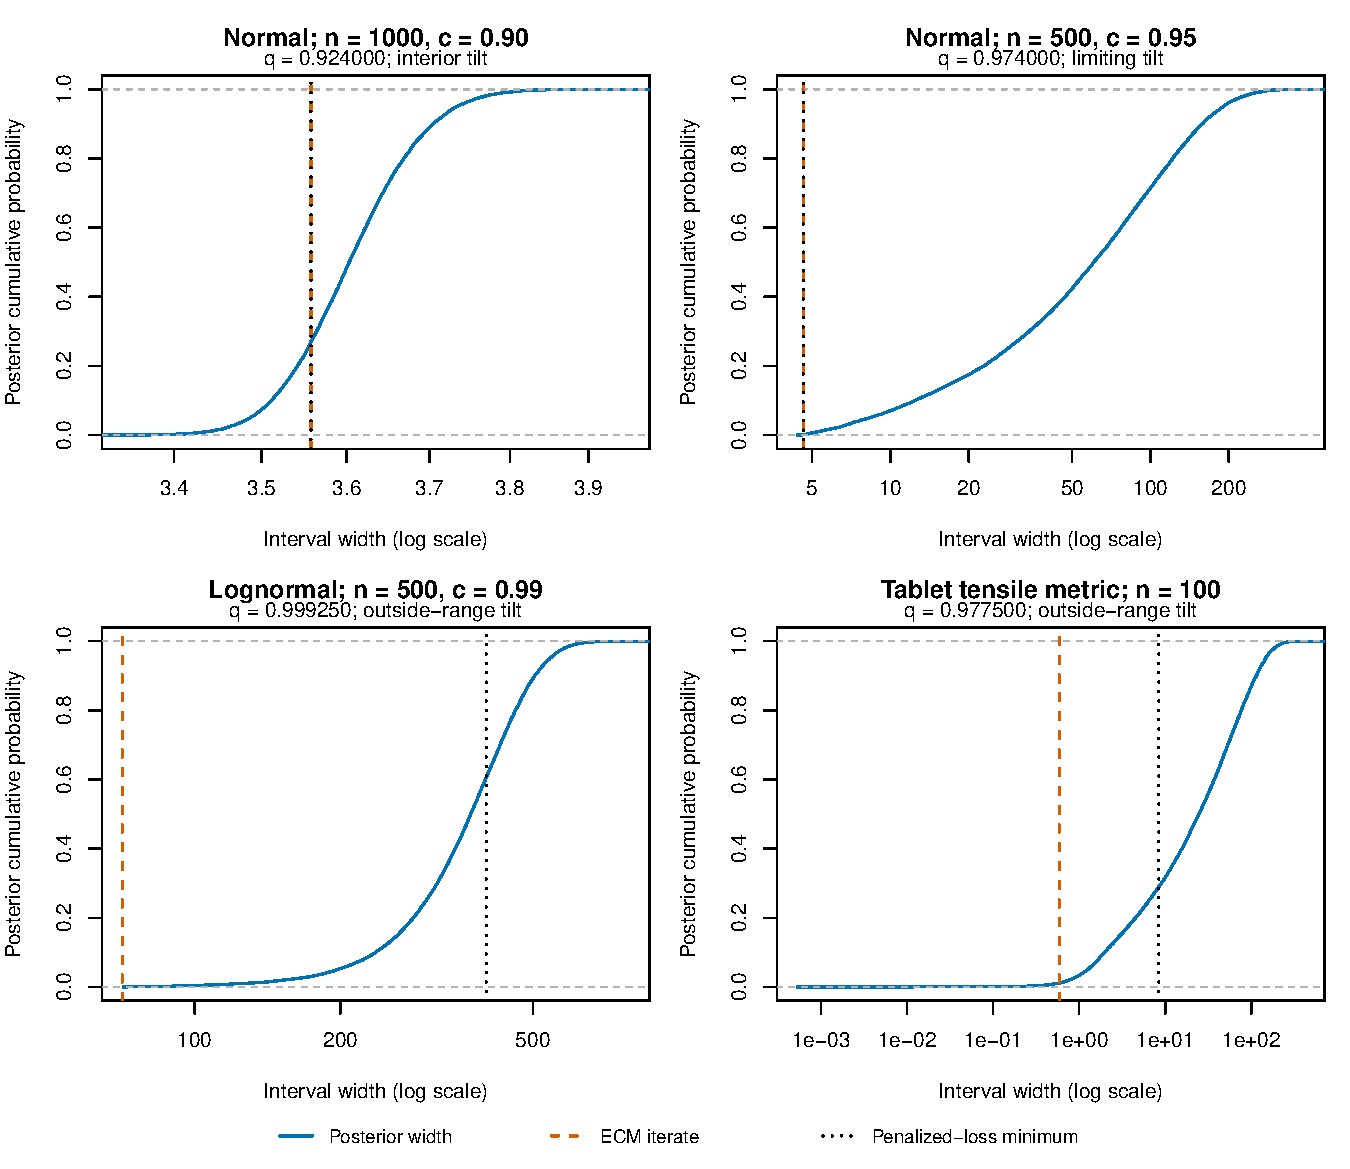
\includegraphics[width=\textwidth]{figures/generated/figS_mti_fixed_target_width.pdf}
\caption{\textbf{Posterior interval width at fixed content and tilt.}
Each curve is the empirical posterior cumulative distribution of width
from four marginal slice-within-Gibbs chains. Vertical lines mark the
archived finite-iteration ECM width and a separately minimized value of
the same penalized loss. All quantities within a panel use the same
observations, fitted content, tilt, learning rate, and root priors. The
horizontal axis is logarithmic; widths remain in the original response
units. The selected examples illustrate interior, limiting, and
outside-range empirical tilts. These are conditional posterior
distributions, distinct from repeated-sampling tolerance assessments.}
\label{fig:supp-mti-posterior-width}
\end{figure}
